\section{Data and methodology}
\label{sec:method}

The search looks for one kind of signal: an unresolved carrier at the
star's own position, narrow compared with a single correlator channel, and
drifting in sky frequency because the transmitter accelerates along the line
of sight. Over a long track its power is spread across many channels, so a
search that treats each channel on its own will miss it. The analysis
de-drifts the data before it measures them.

\subsection{The de-drifted search statistic}
\label{sec:statistic}

Each window's dynamic spectrum is stacked along every trial drift rate
$\dot\nu$. The search statistic is the largest stacked signal-to-noise
ratio anywhere on the resulting channel$\times$drift grid,
%
\begin{equation}
T(\mathbf{x})=\max_{\dot\nu,\;\nu}\;
\frac{\sum_{t} I\!\left(\mathbf{x},t,\nu+\dot\nu t\right)\big/\sigma^{2}(t,\nu)}
     {\left[\sum_{t}1\big/\sigma^{2}(t,\nu)\right]^{1/2}},
\label{eq:tstar}
\end{equation}
%
where $I(\mathbf{x},t,\nu)$ is the spectrum at sky position $\mathbf{x}$
in integration $t$ and channel $\nu$, and $\sigma(t,\nu)$ is the noise scale
there. Equation~\ref{eq:tstar} is the matched filter for a constant-drift
carrier: it adds the signal coherently along the track and divides by the
noise of the stacked spectrum, so $T$ is an absolute signal-to-noise ratio
and not a local contrast. The noise scale is the median absolute deviation
across \NCtrl{} control positions at each integration and each channel ---
local in time and frequency, global in position, and shared by the star and
every control, with the across-position median never subtracted from the
numerator. The statistic is evaluated at one position at a time, identically
at the star and at each control, which is what makes the two comparable.
$T_\star$ denotes its value at the star.

Spectra are extracted at the star's apparent position, never from images.
For each integration and each native channel the pipeline forms the
weighted vector average of the phase-shifted visibilities, in total
intensity: the mean $I=(XX+YY)/2$ of the two parallel-hand
correlations. That average is the dirty-map value at the
extraction position: an amplitude, not a deconvolved flux density, so in
a field with extended emission it is not a point-source measurement. The data are used as the archive delivered them, through ALMA's own
calibration and quality assurance, with their flagging carried through
and with no regridding and no deconvolution. All delivered channels are searched,
with no edge-channel trimming. A per-integration median along the
\emph{frequency} axis removes the continuum; no median is taken along
time, so a one- or two-channel feature cannot be removed by it. One
subtlety matters for every power quoted below. The delivered channels are
smoothed, so a channel's effective noise bandwidth is not its separation,
and flux density times channel width is not yet a radiated power. A
response correction computed from the correlator's own channel shape
supplies the difference. It is derived, and validated against the
effective resolutions ALMA reports, in Appendix~\ref{app:conventions}.

One convention is fixed here and holds everywhere in the paper. The search
itself runs on the topocentric sky frequencies ALMA delivered, and every
drift rate quoted is the apparent one at the telescope, since that is what
the data contain and what a reader can recompute from the released channel
axes. Two steps need the star's own frame rather than the sky's, and both
take it: a crossing is compared with the line catalogue, and a repeat epoch
is read at the predicted cell, after each block's frequency axis has been
corrected for the Earth's motion at that block's epoch and then for the
star's systemic velocity. Nothing in this paper is evaluated in a
barycentric frame alone.

Two power quantities carry the main text. The trigger level $P_{\rm
trig}$ is the equivalent isotropic radiated power,
$\mathrm{EIRP}=4\pi d^{2}S\,\Delta\nu$ at distance $d$, of a carrier that
makes $T_\star$ reach $T_{\rm trig}=\StageNullTrig$ in one native channel
of width $\Delta\nu$. It is an internal pipeline level, the power at
which the search fires, and it is neither a sensitivity nor a
significance. The sensitivity is $\mathrm{EIRP}_{90}$, the power at which
nine injected carriers in ten are recovered through the \emph{complete}
selection of \S\ref{sec:summary}, the spatial ranking requirement included.
It is a recovery fraction through this pipeline, measured rather than
assumed, and it is not the probability of a statistically significant
detection: no stage of the chain carries a calibrated significance, so no
such probability exists to quote. \SelNTone{} synthetic carriers of known
amplitude were injected into calibrated visibilities and recovered
through the unmodified pipeline. They span \SelNUnit{} block--window
configurations, both ALMA arrays, four bands and the sample's full range
of channel widths. For Class~A the result is not a single factor, because
the screen's cost depends on what the control ring contains. Where the ring
is noise --- \StrNNoiseWin{} of the \NWinA{} Class~A windows --- ninety per
cent of carriers are recovered at $\StrMultNoise\,P_{\rm trig}$; in the
\StrNDiscWin{} whose ring carries resolved emission the injected ladder
reaches that point only above $\StrPosCtrl\,P_{\rm trig}$, so those windows
carry a bound rather than a value (\S\ref{sec:pninetysel}). Class~B keeps
one factor, $\EirpNinetyMultB\,P_{\rm trig}$. Every limit quoted in this
paper is the $\mathrm{EIRP}_{90}$ of its own window on its own stratum,
given to two significant figures beside its native channel width; its error
budget is Table~\ref{tab:p90budget}. The absolute flux scale is checked twice from
outside, in two bands on two arrays: the extractor reproduces an
independent reduction of the same AU~Mic visibilities to
\PxJanRatio\,$\pm$\,\PxJanRatioErr, and the published quiescent flux
density of $\epsilon$~Eridani to \PxEpsRatio\,$\pm$\,\PxEpsRatioErr{}
\citep{Burton2022}.

The drift range searched is bounded by an acceleration, not by a
frequency. Drift rate and line-of-sight acceleration are one quantity in
two sets of units, $a_{\rm los}=c\,\dot\nu/\nu$, so a ceiling expressed
as $\dot\nu/\nu$ is the same physical limit in every band. The default
ceiling is \DriftCeilLo--\DriftCeilHi\,Hz\,s$^{-1}$\,GHz$^{-1}$, that is
$|a_{\rm los}|\le\AccelCeilMed$--$\AccelCeilMax$\,m\,s$^{-2}$. That is
the acceleration of a transmitter orbiting a solar-type star at a few
hundredths of an au. It is the \citet{Mason2025} fiducial with a
threefold margin, widened for a confirmed exoplanet host whenever the
innermost known planet demands more. The margin is not cosmetic: at unit
margin the search would have been blind to two of the windows that
produced a crossing. The grid is uniform in $\dot\nu$, and fine enough
that a carrier midway between two trials loses no more than
\DriftGridFineHalf{} of a native channel over the longest track. Two
limits are worth stating plainly. The rates searched are the apparent ones at the
telescope, so a deliberately chirped carrier is not distinguished from an
accelerating platform. And a transmitter need not be bound to a
known planet at all, so drifts faster than the ceiling are simply
unconstrained (Fig.~\ref{fig:accel}).

\begin{figure}
\centering
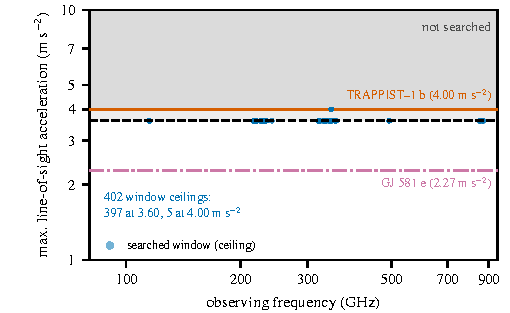
\includegraphics[width=\columnwidth]{figures/drift_acceleration.pdf}
\caption{What the drift search reaches, as a physical selection function.
The drift ceiling of each of the \NWinA{} Class~A windows (points),
converted to line-of-sight acceleration, $|a|=c\,\dot\nu/\nu$, against
observing frequency; the shaded region above is unsearched. The boundary
is flat because the grid was built at constant acceleration; in the units
the search works in it is not, running \AccelDriftLo\,kHz\,s$^{-1}$ at
\AccelFreqLo\,GHz to \AccelDriftHi\,kHz\,s$^{-1}$ at \AccelFreqHi\,GHz.
Horizontal lines are reference accelerations: Earth's rotation
(\AccelEarthRot\,m\,s$^{-2}$ at the equator) and orbit
(\AccelEarthOrb\,m\,s$^{-2}$), and the two most demanding known planets
of any target, \AccelWorstName{} (\AccelWorstVal\,m\,s$^{-2}$) and
\AccelSecondName{} (\AccelSecondVal\,m\,s$^{-2}$). The boundary drawn is
the default ceiling, \AccelCeilMed\,m\,s$^{-2}$, which is also the
median; it runs to \AccelCeilMax\,m\,s$^{-2}$ on the \AccelNWide{}
\AccelWideStar{} windows, and it is each window's own ceiling that
decides whether a given orbit is contained. TRAPPIST-1 transits, so the
edge-on figure is the relevant one for the most demanding case: planet~b
lies above the default ceiling for \TrapPhaseHi{} per cent of its orbital
phase and above the widened one for \TrapPhaseLo{} per cent, and is
searchable through the rest.}
\label{fig:accel}
\end{figure}

Only part of the archive can carry a drift search at all, and the two
classes reported here are that division. Channelisation in the sample is
bimodal, with an empty gap between the modes, so the split is unambiguous.
Class~A is the primary experiment: the \NWinA{} fine-channel windows, median
\ChanAMedKHz\,kHz, in which the maximum searched drift crosses of order one
channel or more over the on-source track ($\eta_{\rm drift} =
|\dot\nu_{\max}|\tau_{\rm track}/\Delta\nu_{\rm ch} \gtrsim 1$), and the
only class with measured end-to-end recovery of a drifting carrier. Class~B
is the secondary experiment: the \NWinB{} coarse-channel windows, mode
\ChanBModeMHz\,MHz, in which a carrier stays inside one channel for the
whole track; these constrain a persistent unresolved spectral excess, carry
no drift discrimination, and are never described as a carrier search here.
Each window's own $\eta_{\rm drift}$, trial-drift count and acceleration
ceiling are released catalogue columns, so a reader may reclassify on the
physical criterion instead; the two criteria do not partition the survey
identically. Results are given per class, and combined only where that is
statistically appropriate.

\subsection{From a crossing to a candidate}
\label{sec:summary}

Every window passes through the same four tests in the same order, and
three words name what comes out of them: a \emph{crossing}, a
\emph{candidate} and, had one survived, a \emph{confirmed} signal
(Fig.~\ref{fig:chain}). Each test is set out below as the quantity it
measures, the number that quantity is compared with, when that number was
fixed, and what passing it does and does not establish. There is no fifth
test, and not one of the four is a significance test.

\begin{enumerate}[label=(\roman*),leftmargin=1.9em,itemsep=3pt,topsep=3pt,parsep=0pt]
\item \emph{Trigger $\to$ a crossing.} The quantity is $T_\star$, the
de-drifted statistic of Eq.~\ref{eq:tstar} read at the stellar position; the
criterion is $T_\star\geq T_{\rm trig}=\StageNullTrig$ in at least one
channel$\times$drift cell; and both the statistic and the level were fixed
before the archival search began. \textbf{$T_{\rm trig}$ is a trigger
threshold and not a detection significance.} $T$ is not shown to follow any
standard distribution under the null, so the level carries no tail
probability, and a window holds between \TuCellsLo{} and $\TuCellsHi$
independent cells, so one level buys very different protection in a coarse
single-pointing window and in a finely channelised one on a long track. A
crossing establishes only that the window goes on to the next three tests.
\item \emph{Line attribution.} The quantity is the crossing's velocity
offset from the nearest transition of a frozen molecular-line catalogue,
evaluated in the star's own rest frame; the criterion is
$\pm\MaskHalfKms$\,km\,s$^{-1}$, inside which the crossing is astrophysical
and goes no further; and the catalogue, the species list and the half-width
were all fixed before any crossing was classified. The half-width follows
the Keplerian line-of-sight velocities of gas surviving beyond a few au,
${\lesssim}13$\,km\,s$^{-1}$, with margin for the systemic velocity. The
mask classifies rather than detects: it is applied after the search, so no
threshold moves and no window goes unsearched. What it establishes is a
kinematic coincidence with a known line, and its price is that the survey
constrains nothing inside the excluded intervals ---
${\approx}\SearchedUnionGHz$\,GHz of the \UnionGHz\,GHz covered survives the
mask (Appendix~\ref{app:linemask}).
\item \emph{Spatial selection $\to$ a candidate.} The quantity is $T_\star$
ranked against the same statistic at \NCtrl{} control positions in the same
window, drawn once from a fixed seed into an annulus placed by each block's
own synthesised and primary beams so that no control sits on the star. The
rank runs the way a competition does: its \emph{lowest} value,
$1/(\NCtrl+1)$, means the star beat every control, so a rank below one half
places the star high in its own field. The criterion is that lowest value,
and the ring, its seed and the criterion were all fixed before any crossing
was inspected. \textbf{This is a localisation and ranking filter, not a
significance test.} The stellar and control positions are not demonstrably
exchangeable, so no per-window false-alarm probability can be attached to
the rank; and the filter responds to compactness rather than to origin. The
clearest demonstration is $\beta$~Pictoris, where genuine carbon monoxide
fails the screen because the resolved disc lifts the control positions along
with the star. \emph{The screen measures compactness rather than
authenticity}, which is why it decides which crossings are examined and
never establishes one. Requiring it costs a factor $\times\ScrCostA$ in
sensitivity, comparing the two blanket figures: $\ScrTrigOnlyA\,P_{\rm
trig}$ at the trigger alone against $\EirpNinetyMultA\,P_{\rm trig}$ through
the screen. Almost all of that is paid in the disc-affected stratum --- where
the ring is noise the cost is only $\times\ScrCostNoise$ --- and every
completeness in this paper is charged for it (Appendix~\ref{app:radius}).
\item \emph{Independent recurrence $\to$ confirmation.} The quantity is
$T_\star$ at the cell the first epoch predicts, read in a later execution
block of the same star at a single drift rate after the frame correction of
\S\ref{sec:statistic}; the criterion is that it reach the trigger again; and
the test was specified before the repeat epochs were searched.
\textbf{This is the survey's only confirmation criterion}, and the archive's
uneven temporal sampling is the main reason it is a weak one: only part of
the sample has epochs separated well enough to apply it at all.
\end{enumerate}

Most crossings are expected by chance, because a fixed threshold is not a
fixed false-alarm rate. The expectation is computed window by window, from
that window's own cell count and the exceedance rate measured at its own
control positions, then summed over the windows searched. It predicts
\RsevChanceExp{} unattributed Class~A crossings against
\RsevChanceObsAUnattr{} observed, about two-thirds of the \NHitsA{} Class~A
crossings. Appendix~\ref{app:falsealarm} gives the conditioning of that
expectation and the control ensemble it is measured on.

The displacement that leaves the rank uncalibrated is measured out of sample
and independently of the crossings: on \HoWin{} windows the frozen pipeline
had never seen, the stellar rank has median \HoRankMed{} where one half is
expected if the star and its controls were interchangeable, and a
parameter-free correction for the annulus geometry does not restore an
exchangeable statistic (Appendix~\ref{app:radius}). Throughout this paper
$p$ denotes a genuine significance level, and no probability computed
against the screen's own null is called one.

Three corrections precede the statistic: the extraction field is chosen so
that the star lies inside the delivered primary-beam field rather than merely
inside the quoted field of view; the stellar position is propagated to the
observation epoch and used as the apparent position; and on-source time is
accounted per integration from the delivered exposure records rather than
from the scan intentions.

A visibility-domain check asks whether a crossing's emission is at the
stellar coordinates rather than elsewhere in the field. It is applied to
every crossing but reported beside the chain rather than inside it, because
it cannot discriminate at the trigger (\S\ref{sec:vistest}).

That the chain finds what it is meant to find is shown twice over: by the
injected carriers above, and by $\beta$~Pictoris CO, a real feature at a
known stellar position, recovered and localised in two transitions and
\NStageOneBpicEb{} execution blocks (\S\ref{sec:bpicval}).

%% HANDOVER (04_method.tex, round 10, r10-stat) -- supersedes the v4.10 note.
%% CLOSED since v4.10: tab_maskladder.tex now exists, so the build no longer
%%   dies on it; app:notation, tab:quantities, tab:p90budget are still not
%%   cited from here, which is intended.
%% STILL OPEN, all queued in /workspace/SETI/referee_r10/INTEGRATION_QUEUE.md:
%%  * (entry 6)  survey_numbers_round130.tex must be \input, before round 103.
%%  * (entry 20) fig:chain prints as Figure 8 but is first cited here in S4.2.
%%               Move the float into this file, or I will host it on request.
%%  * (entry 14) the third correction below still says the stellar position is
%%               "propagated to the observation epoch", which is the sentence
%%               R2-M9 quotes.  It becomes "proper motion and annual parallax
%%               both" the moment r10-sens's re-extraction lands, and not
%%               before -- we must not assert a correction we have not applied.
%%  * (entry 13) the frequency frame is now stated ONCE, here, in the stellar
%%               rest frame for attribution and recurrence.  app_I_linemask.tex
%%               still says the mask is evaluated topocentrically.
%%  * (entry 11) the remaining "5 sigma" trigger phrasings are all outside this
%%               file; this one is clean, measured in the built text with
%%               referee_r10/trigword.py.
%% NUMBERS STILL WANTED here: \EirpNinetyPctLo / \EirpNinetyPctHi (one combined
%%   interval on the multiplier), \SelPNinetyCoarse (a Class B sensitivity,
%%   which the document cannot quote at all today), a macro for the Keplerian
%%   half-width (still typed as 13 km/s in stage (ii)) and one for the threefold
%%   drift margin.
%% fig:funnel's caption in 03_sample.tex still cites \S\ref{sec:summary} for
%%   "the list"; sec:summary is the four-stage chain now, so that clause wants
%%   repointing at Fig.~\ref{fig:chain}.
%% Table 10 (tab:algorithm) in App A remains unreferenced -- both its citations
%%   were here and the four-stage chain replaces it; the appendix owner should
%%   delete the float.
